Recall that for each $k$ the number of \ktypes is finite. Let $\beta_k$ be this
number. Proposition~\ref{prop-nec-implies-LT} is an immediate consequence of
the following proposition.

\begin{prop}\label{lemma-pumping}
  Let $L$ be a \ktame regular tree language. Set $\kappa=\beta_k + k + 1$.
  Then for all $l>\kappa$ and any two trees $t,t'$ if
  \sameblocks{t}{t'}{\kappa} then there exist two trees $T,T'$ with
\begin{enumerate}[\em(1)]
\item $t \in L\ $ ~iff~ $\ T \in L$
\item $t' \in L\ $ ~iff~ $\ T' \in L$
\item \sameblocks{T}{T'}{l}
\end{enumerate}
\end{prop}

\begin{proof}[Proof of Proposition~\ref{prop-nec-implies-LT} using
  Proposition~\ref{lemma-pumping}]
  Assume $L$ is \ktame and let $\kappa$ be defined as in
  Proposition~\ref{lemma-pumping}. We show that $L$ is in LT iff $L$ is
  \testable{\kappa}. Assume $L$ is in LT. Then $L$ is \testable{l} for some $l
  \in \mathbb{N}$. We show that $L$ is actually \testable{\kappa}. For this it
  suffices to show that for any pair of trees $t$ and $t'$, if
  \sameblocks{t}{t'}{\kappa} then $t \in L$ iff $t' \in L$. Let $T$ and $T'$ be
  the trees constructed for $l$ from $t$ and $t'$ by
  Proposition~\ref{lemma-pumping}. We have \sameblocks{T}{T'}{l} and therefore
  $T \in L$ iff $T' \in L$. As we also have $t \in L$ iff $T \in L$ and $t' \in
  L$ iff $T' \in L$, the proposition is proved.
\end{proof}

Before proving Proposition~\ref{lemma-pumping} we need some extra terminology.
A non-empty context $C$ occurring in a tree $t$ is a \emph{loop of \ktype
  $\tau$} if the \ktype of its root and the \ktype of its port is $\tau$. A
non-empty context $C$ occurring in a tree $t$ is a \kloop if there is some
\ktype $\tau$ such that $C$ is a loop of \ktype $\tau$. Given a context $C$ we call the
path from the root of $C$ to its port the \emph{principal path of
  $C$}. Finally, the result of the \emph{insertion} of a \kloop $C$ at a node
$x$ of a tree $t$ is a tree $T$ such that if $t=D \cdot \subtree{t}{x}$ then
$T=D\cdot C \cdot \subtree{t}{x}$. Typically an insertion will occur only when
the \ktype of $x$ is $\tau$ and $C$ is a loop of \ktype $\tau$. In this case
the \ktypes of the nodes initially from $t$ and of the nodes of $C$ are unchanged by this operation.


\begin{proof}[Proof of Proposition~\ref{lemma-pumping}]

  Suppose that $L$ is \ktame. We start by proving two lemmas that will be
  useful in the construction of $T$ and $T'$. Essentially these lemmas show
  that even though being \ktame does not imply being \testable{(k+1)} (recall
  the remark after Theorem~\ref{main-theorem}) some of the expected behavior of
  \testable{(k+1)} languages can still be derived from being \ktame. The first
  lemma shows that given a tree $t$, without affecting membership in $L$, we
  can replace a subtree of $t$ containing only \types{(k+1)} occurring elsewhere
  in $t$ by any other subtree satisfying this property and having the same
  \ktype as root. The second lemma shows the same result for contexts by
  showing that a \kloop can be inserted in a tree $t$ without affecting
  membership in $L$ as soon as all the \types{(k+1)} of the \kloop were
  already present in $t$. After proving these lemmas we will see how to
  combine them for constructing $T$ and $T'$.

\begin{lem}\label{claim-transfer-branch} 
  Assume $L$ is \ktame.  Let $t=Ds$ be a tree where $s$ is a subtree of $t$.
  Let $s'$ be another tree such that the roots of $s$ and $s'$ have the same
  \ktype.

If \lessblocks{s}{D}{k+1} and \lessblocks{s'}{D}{k+1} then
$Ds\in L$ iff $Ds'\in L$.
\end{lem}

\begin{proof}

  We start by proving a special case of the Lemma when $s'$ is actually another
  subtree of $t$. We will use repeatedly this particular case in the proof.

  \begin{claim} \label{claim-transfer-enhanced} Assume $L$ is \ktame. Let $t$
    be a tree and let $x,y$ be two nodes of $t$ not related by the descendant
    relationship and with the same \ktype. We write $s = \subtree{t}{x}$,
    $s' = \subtree{t}{y}$ and $C$ the context such that $t = Cs$.
    If $\lessblocks{s}{C}{k+1}$ then $Cs \in L$ iff $Cs' \in L$.
\end{claim}


\begin{proof} The proof is done by induction on the depth of $s$ and makes
  crucial use of $k$-guarded horizontal transfer.

  Assume first that $s$ is of depth less than $k$. Since $x$ and $y$ have the same
  \ktype, we have $s = s'$ and the result follows.

  Assume now that $s$ is of depth greater than $k$.
 
  Let $\tau$ be the \type{(k+1)} of $x$. We assume that $s$ is a tree of the form
  $a(s_1,s_2)$. Notice that the \ktype of the roots of $s_1$ and $s_2$ are completely determined
  by $\tau$. Since $\lessblocks{s}{C}{k+1}$, there exists a node $z$ in $C$ of
  type $\tau$. We write $s'' = \subtree{t}{z}$.

  We consider several cases depending on the relationship between $x$, $y$ and $z$.
  We first consider the case where $x$ and $z$ are not related by the descendant
  relationship, then we reduce the other cases to this case.

  Assume that $x$ and $z$ are not related by the descendant relationship. Since
  $s''$ is of type $\tau$, it is of the form $a(s''_1,s''_2)$ where the roots
  of $s''_1$ and $s''_2$ have the same \ktype as respectively the roots of
  $s_1$ and $s_2$. By hypothesis all the \types{(k+1)} of $s_1$ and $s_2$
  already appear in $C$ and hence we can apply the induction hypothesis to
  replace $s_1$ by $s''_1$ and $s_2$ by $s''_2$ without affecting membership
  in $L$. Notice that the resulting tree is $Cs''$, that $t=Cs \in L$ iff
  $Cs'' \in L$, and that $Cs''$ contains two copies of the subtree $s''$, one
  at position $x$ and one at position $z$. We now show that we can derive
  $Cs'$ from $Cs''$ using $k$-guarded operations. Since $L$ is \ktame it will
  follow that that $Cs'' \in L$ iff $Cs' \in L$ and thus $Cs \in L$ iff $Cs' \in L$.
  Let $t''=Cs''$ and we distinguish between three cases depending on the relationship between $z$ and $y$ in
  $t''$:


\tikzstyle{arr} = [line width=4pt, ->]
\tikzstyle{bag}=[minimum size=20pt,inner sep=0pt]
\tikzstyle{dot}=[draw,circle,fill,minimum size=4pt,inner sep=0pt]

\begin{enumerate}[(1)]
\item If $z$ is a descendant of $y$, let $D=t''[y,z]$ and notice that $s'=Ds''$. Since $x$, $y$ and $z$ have
  the same \ktype, we use $k$-guarded vertical stutter to duplicate $D$ and a
  $k$-guarded horizontal swap to move the new copy of $D$ at position $x$ (see
  the picture below). The resulting tree is $Cs'$ as desired.


\begin{center}
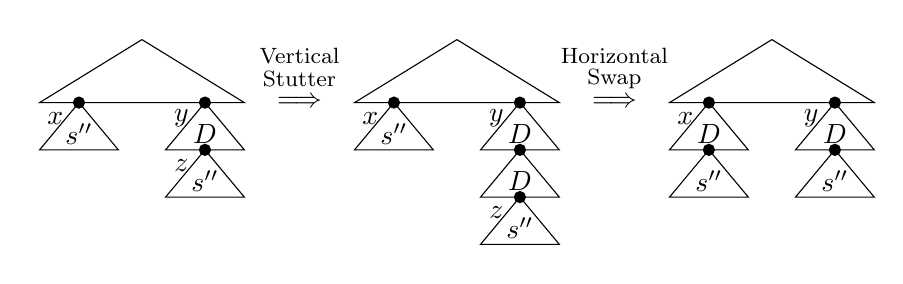
\begin{tikzpicture}

\draw (2.5,2) -- (1.2,1.2) -- (3.8,1.2) -- (2.5,2);

\draw (1.7,1.2) -- (1.2,0.6) -- (2.2,0.6) -- (1.7,1.2);
\node[dot] at (1.7,1.2) {};
\node[bag] at (1.7,0.8) {$s''$};
\node[bag] at (1.4,1.0) {$x$};

\draw (3.3,1.2) -- (2.8,0.6) -- (3.8,0.6) -- (3.3,1.2);
\node[dot] at (3.3,1.2) {};
\draw (3.3,0.6) -- (2.8,0) -- (3.8,0) -- (3.3,0.6);
\node[dot] at (3.3,0.6) {};

\node[bag] at (3.3,0.8) {$D$};
\node[bag] at (3.3,0.2) {$s''$};
\node[bag] at (3.0,1.0) {$y$};
\node[bag] at (3.0,0.4) {$z$};



\node[bag] at (4.5,1.2) {$\Longrightarrow$};
\node[bag] at (4.5,1.8) {\footnotesize Vertical};
\node[bag] at (4.5,1.5) {\footnotesize Stutter};

\draw (6.5,2) -- (5.2,1.2) -- (7.8,1.2) -- (6.5,2);

\draw (5.7,1.2) -- (5.2,0.6) -- (6.2,0.6) -- (5.7,1.2);
\node[dot] at (5.7,1.2) {};
\node[bag] at (5.7,0.8) {$s''$};
\node[bag] at (5.4,1.0) {$x$};


\draw (7.3,1.2) -- (6.8,0.6) -- (7.8,0.6) -- (7.3,1.2);
\node[dot] at (7.3,1.2) {};
\draw (7.3,0.6) -- (6.8,0) -- (7.8,0) -- (7.3,0.6);
\node[dot] at (7.3,0.6) {};
\draw (7.3,0) -- (6.8,-0.6) -- (7.8,-0.6) -- (7.3,0);
\node[dot] at (7.3,0) {};

\node[bag] at (7.3,0.8) {$D$};
\node[bag] at (7.3,0.2) {$D$};
\node[bag] at (7.3,-0.4) {$s''$};
\node[bag] at (7.0,1.0) {$y$};
\node[bag] at (7.0,-0.2) {$z$};


\node[bag] at (8.5,1.2) {$\Longrightarrow$};
\node[bag] at (8.5,1.8) {\footnotesize Horizontal};
\node[bag] at (8.5,1.5) {\footnotesize Swap};


\draw (10.5,2) -- (9.2,1.2) -- (11.8,1.2) -- (10.5,2);

\draw (9.7,1.2) -- (9.2,0.6) -- (10.2,0.6) -- (9.7,1.2);
\node[dot] at (9.7,1.2) {};
\draw (9.7,0.6) -- (9.2,0) -- (10.2,0) -- (9.7,0.6);
\node[dot] at (9.7,0.6) {};

\node[bag] at (9.7,0.8) {$D$};
\node[bag] at (9.7,0.2) {$s''$};
\node[bag] at (9.4,1.0) {$x$};

\draw (11.3,1.2) -- (10.8,0.6) -- (11.8,0.6) -- (11.3,1.2);
\node[dot] at (11.3,1.2) {};
\draw (11.3,0.6) -- (10.8,0) -- (11.8,0) -- (11.3,0.6);
\node[dot] at (11.3,0.6) {};

\node[bag] at (11.3,0.8) {$D$};
\node[bag] at (11.3,0.2) {$s''$};
\node[bag] at (11.0,1.0) {$y$};

\end{tikzpicture}
\end{center}


\item If $z$ is an ancestor of $y$, let $D=t''[z,y]$ and notice that $s''=Ds'$. Since $y$ and $x$ have the
  same \ktype, we use $k$-guarded horizontal swap followed by a $k$-guarded vertical
  stutter to delete the copy of $D$ (see the picture below). The resulting tree is
  $Cs'$ as desired.


\begin{center}
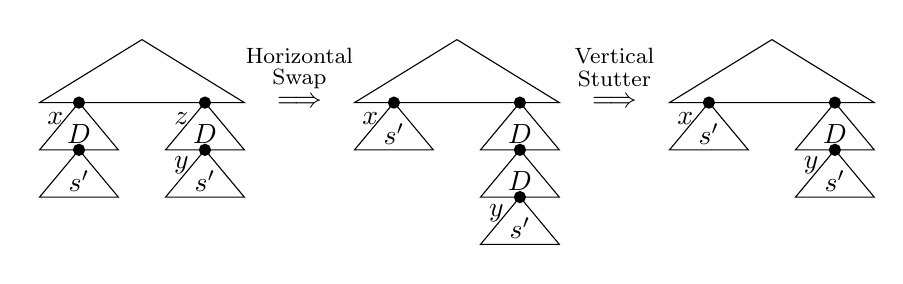
\begin{tikzpicture}


\draw (2.5,2) -- (1.2,1.2) -- (3.8,1.2) -- (2.5,2);

\draw (1.7,1.2) -- (1.2,0.6) -- (2.2,0.6) -- (1.7,1.2);
\node[dot] at (1.7,1.2) {};
\draw (1.7,0.6) -- (1.2,0) -- (2.2,0) -- (1.7,0.6);
\node[dot] at (1.7,0.6) {};

\node[bag] at (1.7,0.8) {$D$};
\node[bag] at (1.7,0.2) {$s'$};
\node[bag] at (1.4,1.0) {$x$};

\draw (3.3,1.2) -- (2.8,0.6) -- (3.8,0.6) -- (3.3,1.2);
\node[dot] at (3.3,1.2) {};
\draw (3.3,0.6) -- (2.8,0) -- (3.8,0) -- (3.3,0.6);
\node[dot] at (3.3,0.6) {};

\node[bag] at (3.3,0.8) {$D$};
\node[bag] at (3.0,0.4) {$y$};
\node[bag] at (3.3,0.2) {$s'$};
\node[bag] at (3.0,1.0) {$z$};


\node[bag] at (4.5,1.2) {$\Longrightarrow$};
\node[bag] at (4.5,1.8) {\footnotesize Horizontal};
\node[bag] at (4.5,1.5) {\footnotesize Swap};

\draw (6.5,2) -- (5.2,1.2) -- (7.8,1.2) -- (6.5,2);

\draw (5.7,1.2) -- (5.2,0.6) -- (6.2,0.6) -- (5.7,1.2);
\node[dot] at (5.7,1.2) {};
\node[bag] at (5.7,0.8) {$s'$};
\node[bag] at (5.4,1.0) {$x$};


\draw (7.3,1.2) -- (6.8,0.6) -- (7.8,0.6) -- (7.3,1.2);
\node[dot] at (7.3,1.2) {};
\draw (7.3,0.6) -- (6.8,0) -- (7.8,0) -- (7.3,0.6);
\node[dot] at (7.3,0.6) {};
\draw (7.3,0) -- (6.8,-0.6) -- (7.8,-0.6) -- (7.3,0);
\node[dot] at (7.3,0) {};

\node[bag] at (7.3,0.8) {$D$};
\node[bag] at (7.3,0.2) {$D$};
\node[bag] at (7.3,-0.4) {$s'$};
\node[bag] at (7.0,-0.2) {$y$};


\node[bag] at (8.5,1.2) {$\Longrightarrow$};
\node[bag] at (8.5,1.8) {\footnotesize Vertical};
\node[bag] at (8.5,1.5) {\footnotesize Stutter};





\draw (10.5,2) -- (9.2,1.2) -- (11.8,1.2) -- (10.5,2);

\draw (9.7,1.2) -- (9.2,0.6) -- (10.2,0.6) -- (9.7,1.2);
\node[dot] at (9.7,1.2) {};
\node[bag] at (9.7,0.8) {$s'$};
\node[bag] at (9.4,1.0) {$x$};

\draw (11.3,1.2) -- (10.8,0.6) -- (11.8,0.6) -- (11.3,1.2);
\node[dot] at (11.3,1.2) {};
\draw (11.3,0.6) -- (10.8,0) -- (11.8,0) -- (11.3,0.6);
\node[dot] at (11.3,0.6) {};

\node[bag] at (11.3,0.8) {$D$};
\node[bag] at (11.3,0.2) {$s'$};
\node[bag] at (11.0,0.4) {$y$};

\end{tikzpicture}
\end{center}


\item If $z$ and $y$ are not related by the descendant relation, then $x$,
 $y$ and $z$ have the same \ktype and $\subtree{t''}{x} = \subtree{t''}{z}$.
 We use $k$-guarded horizontal transfer to replace \subtree{t''}{x} with
 \subtree{t''}{y} as depicted below.

\begin{center}
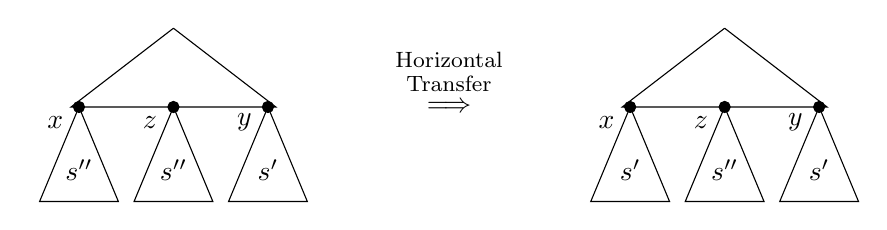
\begin{tikzpicture}

\draw (1.5,2.2) -- (0.2,1.2) -- (2.8,1.2) -- (1.5,2.2);

\draw (0.3,1.2) -- (-0.2,0) -- (0.8,0) -- (0.3,1.2);

\node[bag] at (0.3,0.4) {$s''$};
\node[bag] at (0,1.0) {$x$};
\node[dot] at (0.3,1.2) {};


\draw (1.5,1.2) -- (1.0,0) -- (2.0,0) -- (1.5,1.2);

\node[bag] at (1.5,0.4) {$s''$};
\node[bag] at (1.2,1.0) {$z$};
\node[dot] at (1.5,1.2) {};

\draw (2.7,1.2) -- (2.2,0) -- (3.2,0) -- (2.7,1.2);

\node[bag] at (2.7,0.4) {$s'$};
\node[bag] at (2.4,1.0) {$y$};
\node[dot] at (2.7,1.2) {};


\node[bag] at (5.0,1.2) {$\Longrightarrow$};
\node[bag] at (5.0,1.8) {\footnotesize Horizontal};
\node[bag] at (5.0,1.5) {\footnotesize Transfer};


\draw (8.5,2.2) -- (7.2,1.2) -- (9.8,1.2) -- (8.5,2.2);

\draw (7.3,1.2) -- (6.8,0) -- (7.8,0) -- (7.3,1.2);

\node[bag] at (7.3,0.4) {$s'$};
\node[bag] at (7,1.0) {$x$};
\node[dot] at (7.3,1.2) {};


\draw (8.5,1.2) -- (8.0,0) -- (9.0,0) -- (8.5,1.2);

\node[bag] at (8.5,0.4) {$s''$};
\node[bag] at (8.2,1.0) {$z$};
\node[dot] at (8.5,1.2) {};

\draw (9.7,1.2) -- (9.2,0) -- (10.2,0) -- (9.7,1.2);

\node[bag] at (9.7,0.4) {$s'$};
\node[bag] at (9.4,1.0) {$y$};
\node[dot] at (9.7,1.2) {};



\end{tikzpicture}
\end{center}


\end{enumerate}

\bigskip 

This concludes the case where $x$ and $z$ are not related by the descendant
relationship in $t$. We are left with the case where $x$ is a descendant of
$z$ (recall that $z$ is outside $s$ and therefore not a descendant of $x$).
We reduce this problem to the previous case by considering two subcases:

\begin{iteMize}{$\bullet$}

\item If $y,z$ are not related by the descendant relationship, we use a
  $k$-guarded horizontal swap to replace $s$ by $s'$ and vice versa. This
  reverses the roles of $x$ and $y$ and as $y$ and $z$ are not related by
  the descendant relationship and position $y$ now has \type{(k+1)} $\tau$
  we can apply the previous case.

\begin{center}
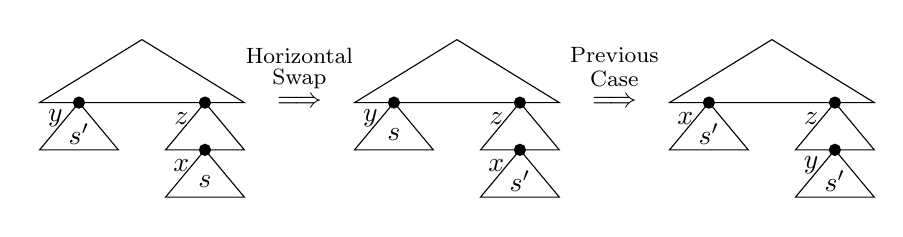
\begin{tikzpicture}

\draw (2.5,2) -- (1.2,1.2) -- (3.8,1.2) -- (2.5,2);


\draw (1.7,1.2) -- (1.2,0.6) -- (2.2,0.6) -- (1.7,1.2);
\node[dot] at (1.7,1.2) {};
\node[bag] at (1.7,0.8) {$s'$};
\node[bag] at (1.4,1.0) {$y$};

\draw (3.3,1.2) -- (2.8,0.6) -- (3.8,0.6) -- (3.3,1.2);
\node[dot] at (3.3,1.2) {};
\draw (3.3,0.6) -- (2.8,0) -- (3.8,0) -- (3.3,0.6);
\node[dot] at (3.3,0.6) {};

\node[bag] at (3.3,0.2) {$s$};
\node[bag] at (3.0,1.0) {$z$};
\node[bag] at (3.0,0.4) {$x$};



\node[bag] at (4.5,1.2) {$\Longrightarrow$};
\node[bag] at (4.5,1.8) {\footnotesize Horizontal};
\node[bag] at (4.5,1.5) {\footnotesize Swap};


\begin{scope}[xshift=4cm]


\draw (2.5,2) -- (1.2,1.2) -- (3.8,1.2) -- (2.5,2);


\draw (1.7,1.2) -- (1.2,0.6) -- (2.2,0.6) -- (1.7,1.2);
\node[dot] at (1.7,1.2) {};
\node[bag] at (1.7,0.8) {$s$};
\node[bag] at (1.4,1.0) {$y$};

\draw (3.3,1.2) -- (2.8,0.6) -- (3.8,0.6) -- (3.3,1.2);
\node[dot] at (3.3,1.2) {};
\draw (3.3,0.6) -- (2.8,0) -- (3.8,0) -- (3.3,0.6);
\node[dot] at (3.3,0.6) {};

\node[bag] at (3.3,0.2) {$s'$};
\node[bag] at (3.0,1.0) {$z$};
\node[bag] at (3.0,0.4) {$x$};

\end{scope}



\node[bag] at (8.5,1.2) {$\Longrightarrow$};
\node[bag] at (8.5,1.8) {\footnotesize Previous};
\node[bag] at (8.5,1.5) {\footnotesize Case};

\begin{scope}[xshift=8cm]


\draw (2.5,2) -- (1.2,1.2) -- (3.8,1.2) -- (2.5,2);


\draw (1.7,1.2) -- (1.2,0.6) -- (2.2,0.6) -- (1.7,1.2);
\node[dot] at (1.7,1.2) {};
\node[bag] at (1.7,0.8) {$s'$};
\node[bag] at (1.4,1.0) {$x$};

\draw (3.3,1.2) -- (2.8,0.6) -- (3.8,0.6) -- (3.3,1.2);
\node[dot] at (3.3,1.2) {};
\draw (3.3,0.6) -- (2.8,0) -- (3.8,0) -- (3.3,0.6);
\node[dot] at (3.3,0.6) {};

\node[bag] at (3.3,0.2) {$s'$};
\node[bag] at (3.0,1.0) {$z$};
\node[bag] at (3.0,0.4) {$y$};

\end{scope}
\end{tikzpicture}
\end{center}

\item If $z$ is an ancestor of both $x$ and $y$ we use $k$-guarded vertical
  stutter to duplicate the context between $z$ and $x$. This introduces a new
  node $z'$ of type $\tau$ that is not related to $y$ by the descendant
  relationship and we are back in the previous case.

\end{iteMize}

\begin{center}
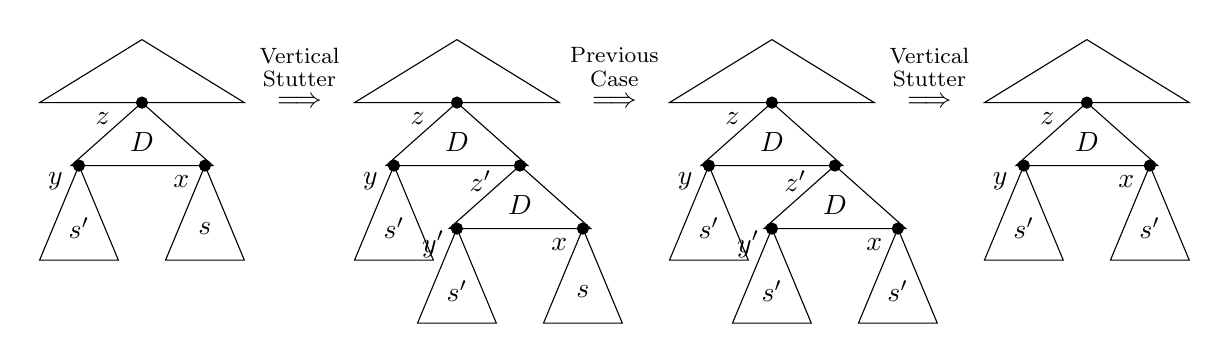
\begin{tikzpicture}

\draw (2.5,2) -- (1.2,1.2) -- (3.8,1.2) -- (2.5,2);

\draw (2.5,1.2) -- (1.6,0.4) -- (3.4,0.4) -- (2.5,1.2);
\node[dot] at (2.5,1.2) {};
\node[bag] at (2.5,0.7) {$D$};
\node[bag] at (2.0,1.0) {$z$};


\draw (1.7,0.4) -- (1.2,-0.8) -- (2.2,-0.8) -- (1.7,0.4);
\node[dot] at (1.7,0.4) {};
\node[bag] at (1.7,-0.4) {$s'$};
\node[bag] at (1.4,0.2) {$y$};

\draw (3.3,0.4) -- (2.8,-0.8) -- (3.8,-0.8) -- (3.3,0.4);
\node[dot] at (3.3,0.4) {};


\node[bag] at (3.3,-0.4) {$s$};
\node[bag] at (3.0,0.2) {$x$};

\node[bag] at (4.5,1.2) {$\Longrightarrow$};
\node[bag] at (4.5,1.8) {\footnotesize Vertical};
\node[bag] at (4.5,1.5) {\footnotesize Stutter};


\begin{scope}[xshift=4cm]
\draw (2.5,2) -- (1.2,1.2) -- (3.8,1.2) -- (2.5,2);

\draw (2.5,1.2) -- (1.6,0.4) -- (3.4,0.4) -- (2.5,1.2);
\node[dot] at (2.5,1.2) {};
\node[bag] at (2.5,0.7) {$D$};
\node[bag] at (2.0,1.0) {$z$};


\draw (1.7,0.4) -- (1.2,-0.8) -- (2.2,-0.8) -- (1.7,0.4);
\node[dot] at (1.7,0.4) {};
\node[bag] at (1.7,-0.4) {$s'$};
\node[bag] at (1.4,0.2) {$y$};

\end{scope}

\begin{scope}[xshift=4.8cm,yshift=-0.8cm]
\draw (2.5,1.2) -- (1.6,0.4) -- (3.4,0.4) -- (2.5,1.2);
\node[dot] at (2.5,1.2) {};
\node[bag] at (2.5,0.7) {$D$};
\node[bag] at (2.0,1.0) {$z'$};


\draw (1.7,0.4) -- (1.2,-0.8) -- (2.2,-0.8) -- (1.7,0.4);
\node[dot] at (1.7,0.4) {};
\node[bag] at (1.7,-0.4) {$s'$};
\node[bag] at (1.4,0.2) {$y'$};

\draw (3.3,0.4) -- (2.8,-0.8) -- (3.8,-0.8) -- (3.3,0.4);
\node[dot] at (3.3,0.4) {};


\node[bag] at (3.3,-0.4) {$s$};
\node[bag] at (3.0,0.2) {$x$};

\end{scope}

\node[bag] at (8.5,1.2) {$\Longrightarrow$};
\node[bag] at (8.5,1.8) {\footnotesize Previous};
\node[bag] at (8.5,1.5) {\footnotesize Case};

\begin{scope}[xshift=8cm]
\draw (2.5,2) -- (1.2,1.2) -- (3.8,1.2) -- (2.5,2);

\draw (2.5,1.2) -- (1.6,0.4) -- (3.4,0.4) -- (2.5,1.2);
\node[dot] at (2.5,1.2) {};
\node[bag] at (2.5,0.7) {$D$};
\node[bag] at (2.0,1.0) {$z$};


\draw (1.7,0.4) -- (1.2,-0.8) -- (2.2,-0.8) -- (1.7,0.4);
\node[dot] at (1.7,0.4) {};
\node[bag] at (1.7,-0.4) {$s'$};
\node[bag] at (1.4,0.2) {$y$};

\end{scope}

\begin{scope}[xshift=8.8cm,yshift=-0.8cm]
\draw (2.5,1.2) -- (1.6,0.4) -- (3.4,0.4) -- (2.5,1.2);
\node[dot] at (2.5,1.2) {};
\node[bag] at (2.5,0.7) {$D$};
\node[bag] at (2.0,1.0) {$z'$};


\draw (1.7,0.4) -- (1.2,-0.8) -- (2.2,-0.8) -- (1.7,0.4);
\node[dot] at (1.7,0.4) {};
\node[bag] at (1.7,-0.4) {$s'$};
\node[bag] at (1.4,0.2) {$y'$};

\draw (3.3,0.4) -- (2.8,-0.8) -- (3.8,-0.8) -- (3.3,0.4);
\node[dot] at (3.3,0.4) {};


\node[bag] at (3.3,-0.4) {$s'$};
\node[bag] at (3.0,0.2) {$x$};

\end{scope}

\node[bag] at (12.5,1.2) {$\Longrightarrow$};
\node[bag] at (12.5,1.8) {\footnotesize Vertical};
\node[bag] at (12.5,1.5) {\footnotesize Stutter};

\begin{scope}[xshift=12cm]
\draw (2.5,2) -- (1.2,1.2) -- (3.8,1.2) -- (2.5,2);

\draw (2.5,1.2) -- (1.6,0.4) -- (3.4,0.4) -- (2.5,1.2);
\node[dot] at (2.5,1.2) {};
\node[bag] at (2.5,0.7) {$D$};
\node[bag] at (2.0,1.0) {$z$};


\draw (1.7,0.4) -- (1.2,-0.8) -- (2.2,-0.8) -- (1.7,0.4);
\node[dot] at (1.7,0.4) {};
\node[bag] at (1.7,-0.4) {$s'$};
\node[bag] at (1.4,0.2) {$y$};

\draw (3.3,0.4) -- (2.8,-0.8) -- (3.8,-0.8) -- (3.3,0.4);
\node[dot] at (3.3,0.4) {};


\node[bag] at (3.3,-0.4) {$s'$};
\node[bag] at (3.0,0.2) {$x$};

\end{scope}

\end{tikzpicture}
\end{center}

\end{proof}

  We now turn to the proof of Lemma~\ref{claim-transfer-branch}. The proof is
  done by induction on the depth of $s'$. The idea is to replace  $s$ with $s'$
  node by node.

  Assume first that $s'$ is of depth less than $k$. Then because the \ktype of
  the roots of $s$ and $s'$ are equal, we have $s=s'$ and the result follows.

  Assume now that $s'$ is of depth greater than $k$. 

  Let $x$ be the node of $t$ corresponding to the root of $s$. Let $\tau$ be
  the \type{(k+1)} of the root of $s'$. We assume that $s'$ is a tree of the
  form $a(s'_1,s'_2)$. Notice that the \ktype of the roots of $s'_1$ and $s'_2$
  are completely determined by $\tau$. By hypothesis \lessblocks{s'}{D}{k+1},
  hence there exists a node $y$ in $D$ of type $\tau$. We consider two
  cases depending on the relationship between $x$ and $y$.

\tikzstyle{arr} = [line width=4pt, ->]
\tikzstyle{bag}=[minimum size=20pt,inner sep=0pt]
\tikzstyle{inner}=[draw,circle,inner sep=0pt]
\tikzstyle{dot}=[draw,circle,fill,minimum size=4pt,inner sep=0pt]

\begin{iteMize}{$\bullet$}
\item If $y$ is an ancestor of $x$, let $E$ be $t[y,x]$ and notice that $x$ and
  $y$ have the same \ktype. This case is depicted below. Hence applying a $k$-guarded vertical stutter we
  can duplicate $E$ obtaining the tree $DEs$. Because $L$ is \ktame, $DEs \in
  L$ iff $t=Ds \in L$. Now the root of $Es$ in $DEs$ is of type $\tau$ and therefore of
  the form $a(s_1,s_2)$ where the roots of $s_1$ and $s_2$ have the same \ktype
  as respectively the roots of $s'_1$ and $s'_2$. By construction all the
  \types{(k+1)} of $s_1$ and $s_2$ already appear in $D$ and hence we can apply
  the induction hypothesis to replace $s_1$ by $s'_1$ and $s_2$ by $s'_2$
  without affecting membership in $L$. Altogether this gives the desired
  result.
\begin{center}
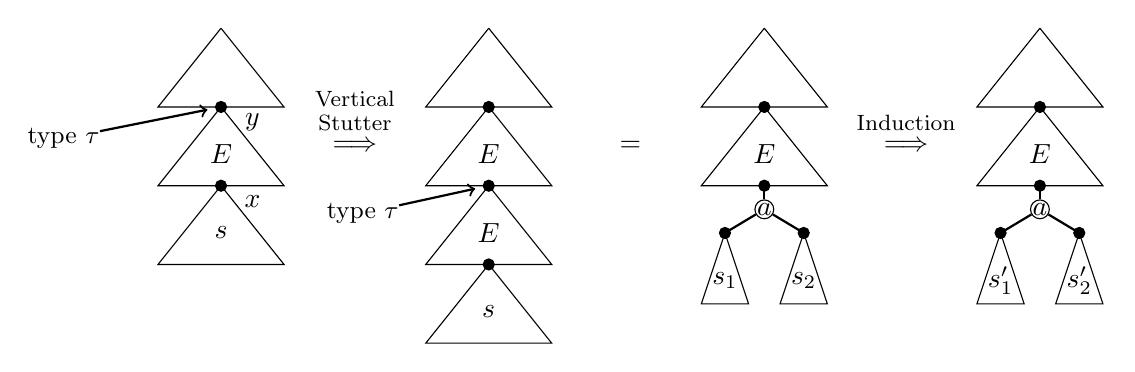
\begin{tikzpicture}

\draw (0.8,2) -- (0,1) -- (1.6,1) -- (0.8,2);
\draw (0.8,1) -- (0,0) -- (1.6,0) -- (0.8,1);
\draw (0.8,0) -- (0,-1) -- (1.6,-1) -- (0.8,0);

\node[dot] at (0.8,1) {};
\node[bag] at (1.2,0.8) {$y$};
\node[dot] at (0.8,0) {};
\node[bag] at (1.2,-0.2) {$x$};

\node[bag] at (0.8,0.4) {$E$};
\node[bag] at (0.8,-0.6) {$s$};

\node[bag] (type1) at (-1.2,0.6) {\small type $\tau$};

\draw[->,shorten >=5pt, thick] (type1) -> (0.8,1);

\node[bag] at (2.5,1.1){\footnotesize Vertical};
\node[bag] at (2.5,0.8){\footnotesize Stutter};
\node[bag] at (2.5,0.5){$\Longrightarrow$};

\draw (4.2,2) -- (3.4,1) -- (5,1) -- (4.2,2);
\draw (4.2,1) -- (3.4,0) -- (5,0) -- (4.2,1);
\draw (4.2,0) -- (3.4,-1) -- (5,-1) -- (4.2,0);
\draw (4.2,-1) -- (3.4,-2) -- (5,-2) -- (4.2,-1);

\node[dot] at (4.2,1) {};
\node[bag] at (4.2,0.4) {$E$};
\node[dot] at (4.2,0) {};
\node[bag] at (4.2,-0.6) {$E$};
\node[dot] at (4.2,-1) {};
\node[bag] at (4.2,-1.6) {$s$};

\node[bag] (type2) at (2.6,-0.35) {\small type $\tau$};

\draw[->,shorten >=5pt, thick] (type2) -> (4.2,0);

\begin{scope}[xshift=3.5cm]

\node[bag] at (2.5,0.5){$=$};

\draw (4.2,2) -- (3.4,1) -- (5,1) -- (4.2,2);
\draw (4.2,1) -- (3.4,0) -- (5,0) -- (4.2,1);

\draw (3.7,-0.6) -- (3.4,-1.5) -- (4.0,-1.5) -- (3.7,-0.6);
\draw (4.7,-0.6) -- (4.4,-1.5) -- (5,-1.5) -- (4.7,-0.6);

\node[bag] at (3.7,-1.2) {$s_1$};
\node[bag] at (4.7,-1.2) {$s_2$};

\node[dot] at (4.2,1) {};
\node[bag] at (4.2,0.4) {$E$};
\node[dot] at (4.2,0) {};
\node[inner] (a) at (4.2,-0.3) {$a$};

\node[dot] at (3.7,-0.6) {};
\node[dot] at (4.7,-0.6) {};

\draw[thick] (a) -- (3.7,-0.6);
\draw[thick] (a) -- (4.7,-0.6);
\draw[thick] (a) -- (4.2,0);


\end{scope}

\begin{scope}[xshift=7cm]

\node[bag] at (2.5,0.8){\footnotesize Induction};
\node[bag] at (2.5,0.5){$\Longrightarrow$};

\draw (4.2,2) -- (3.4,1) -- (5,1) -- (4.2,2);
\draw (4.2,1) -- (3.4,0) -- (5,0) -- (4.2,1);

\draw (3.7,-0.6) -- (3.4,-1.5) -- (4.0,-1.5) -- (3.7,-0.6);
\draw (4.7,-0.6) -- (4.4,-1.5) -- (5,-1.5) -- (4.7,-0.6);

\node[bag] at (3.7,-1.2) {$s'_1$};
\node[bag] at (4.7,-1.2) {$s'_2$};

\node[dot] at (4.2,1) {};
\node[bag] at (4.2,0.4) {$E$};
\node[dot] at (4.2,0) {};
\node[inner] (a) at (4.2,-0.3) {$a$};

\node[dot] at (3.7,-0.6) {};
\node[dot] at (4.7,-0.6) {};

\draw[thick] (a) -- (3.7,-0.6);
\draw[thick] (a) -- (4.7,-0.6);
\draw[thick] (a) -- (4.2,0);

\end{scope}

\end{tikzpicture}
\end{center}

\item Assume now that $x$ and $y$ are not related by the descendant
  relationship. This case is depicted below. Let $s''$ be the subtree of $Ds$ rooted at $y$.  By hypothesis
  all the \types{(k+1)} of $s$ are already present in $D$ and the roots of $s$
  and $s''$ have the same \ktype. Hence we can apply
  Claim~\ref{claim-transfer-enhanced} and we have $Ds \in L$ iff $Ds'' \in L$.
  Now the root of $s''$ is by construction of type $\tau$. Hence $s''$ is
  of the form $a(s_1,s_2)$ where $s_1$ and $s_2$ have all their \types{(k+1)}
  appearing in $D$ and their roots have the same \ktype as respectively
  $s'_1$ and $s'_2$. Hence by induction $s_1$ can be replaced by $s'_1$ and
  $s_2$ by $s'_2$ without affecting membership in $L$. Altogether this gives
  the desired result.

\begin{center}
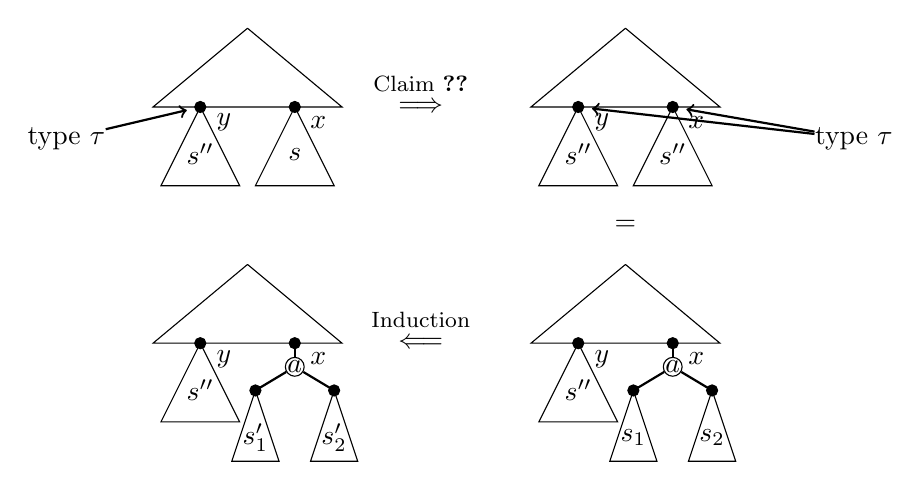
\begin{tikzpicture}

\draw (0.8,2) -- (-0.4,1) -- (2,1) -- (0.8,2);
\draw (0.2,1) -- (-0.3,0) -- (0.7,0) -- (0.2,1);
\draw (1.4,1) -- (0.9,0) -- (1.9,0) -- (1.4,1);

\node[dot] at (0.2,1) {};
\node[bag] at (0.5,0.8) {$y$};
\node[dot] at (1.4,1) {};
\node[bag] at (1.7,0.8) {$x$};

\node[bag] at (0.2,0.4) {$s''$};
\node[bag] at (1.4,0.4) {$s$};

\node[bag] (type1) at (-1.5,0.6) {type $\tau$};

\draw[->,shorten >=5pt, thick] (type1) -> (0.2,1);

\node[bag] at (3,1.3){\footnotesize Claim~\ref{claim-transfer-enhanced}};
\node[bag] at (3,1){$\Longrightarrow$};

\draw (5.6,2) -- (4.4,1) -- (6.8,1) -- (5.6,2);
\draw (5,1) -- (4.5,0) -- (5.5,0) -- (5,1);
\draw (6.2,1) -- (5.7,0) -- (6.7,0) -- (6.2,1);

\node[dot] at (5,1) {};
\node[bag] at (5.3,0.8) {$y$};
\node[dot] at (6.2,1) {};
\node[bag] at (6.5,0.8) {$x$};

\node[bag] at (5,0.4) {$s''$};
\node[bag] at (6.2,0.4) {$s''$};

\node[bag] (type2) at (8.5,0.6) {type $\tau$};

\draw[->,shorten >=5pt, thick] (type2) -> (5,1);
\draw[->,shorten >=5pt, thick] (type2) -> (6.2,1);

\node[bag] at (5.6,-0.5){$=$};



\begin{scope}[yshift=-3cm]

\draw (0.8,2) -- (-0.4,1) -- (2,1) -- (0.8,2);
\draw (0.2,1) -- (-0.3,0) -- (0.7,0) -- (0.2,1);


\node[dot] at (0.2,1) {};
\node[bag] at (0.5,0.8) {$y$};
\node[dot] at (1.4,1) {};
\node[bag] at (1.7,0.8) {$x$};

\node[bag] at (0.2,0.4) {$s''$};

\begin{scope} [xshift=-2.8cm,yshift=1cm]

\draw (3.7,-0.6) -- (3.4,-1.5) -- (4.0,-1.5) -- (3.7,-0.6);
\draw (4.7,-0.6) -- (4.4,-1.5) -- (5,-1.5) -- (4.7,-0.6);

\node[bag] at (3.7,-1.2) {$s'_1$};
\node[bag] at (4.7,-1.2) {$s'_2$};

\node[inner] (a) at (4.2,-0.3) {$a$};

\node[dot] at (3.7,-0.6) {};
\node[dot] at (4.7,-0.6) {};

\draw[thick] (a) -- (3.7,-0.6);
\draw[thick] (a) -- (4.7,-0.6);
\draw[thick] (a) -- (4.2,0);
\end{scope}

\node[bag] at (3,1.3){\footnotesize Induction};
\node[bag] at (3,1){$\Longleftarrow$};

\draw (5.6,2) -- (4.4,1) -- (6.8,1) -- (5.6,2);
\draw (5,1) -- (4.5,0) -- (5.5,0) -- (5,1);

\node[dot] at (5,1) {};
\node[bag] at (5.3,0.8) {$y$};
\node[dot] at (6.2,1) {};
\node[bag] at (6.5,0.8) {$x$};

\node[bag] at (5,0.4) {$s''$};

\begin{scope} [xshift=2cm,yshift=1cm]

\draw (3.7,-0.6) -- (3.4,-1.5) -- (4.0,-1.5) -- (3.7,-0.6);
\draw (4.7,-0.6) -- (4.4,-1.5) -- (5,-1.5) -- (4.7,-0.6);

\node[bag] at (3.7,-1.2) {$s_1$};
\node[bag] at (4.7,-1.2) {$s_2$};

\node[inner] (a) at (4.2,-0.3) {$a$};

\node[dot] at (3.7,-0.6) {};
\node[dot] at (4.7,-0.6) {};

\draw[thick] (a) -- (3.7,-0.6);
\draw[thick] (a) -- (4.7,-0.6);
\draw[thick] (a) -- (4.2,0);
\end{scope}
\end{scope}

\end{tikzpicture}
\end{center}
\end{iteMize}
\end{proof}

We now prove a similar result for \kloops.

\begin{lem}\label{lemma-insert-loop}
  Assume $L$ is \ktame. Let $t$ be a tree and $x$ a node of $t$ of \ktype
  $\tau$. Let $t'$ be another tree such that \sameblocks{t}{t'}{k+1} and $C$ be
  a \kloop of type $\tau$ in $t'$. Consider the tree $T$ constructed from $t$
  by inserting a copy of $C$ at $x$. Then $t \in L$ iff $T \in L$.
\end{lem}

\begin{proof} 

The proof is done in two steps. First we use the \ktame property
  of $L$ to show that we can insert a \kloop $C'$ at $x$ in $t$ such that the
  principal path of $C$ is the same as the principal path of $C'$. By this we
  mean that there is a bijection from the principal path of $C'$ to the
  principal path of $C$ that preserves the child relation and \types{(k+1)}.  In a second step we
  replace one by one the subtrees hanging from the principal path of $C'$ with
  the corresponding subtrees in $C$.

  First some terminology. Given two nodes $y,y'$ of some tree $T$, we say that
  $y'$ is a {\bf l}-ancestor of $y$ if $y$ is a descendant of the left child of
  $y'$. Similarly we define {\bf r}-ancestorship.

  Consider the context $C$ occurring in $t'$. Let $y_{0}, \cdots,y_{n}$ be the
  nodes of $t'$ on the principal path of $C$ and $\tau_{0}, \cdots,\tau_{n}$ be
  their respective \type{(k+1)}. For $0 \leq i < n$, set $c_i$ to {\bf l}
  if $y_{i+1}$ is a left child of $y_i$ and {\bf r} otherwise.

  From $t$ we construct using $k$-guarded swaps and $k$-vertical stutters a
  tree $t_1$ such that there is a sequence of nodes $x_0,\cdots,x_n$ in $t_1$
  with for all $0\leq i < n$, $x_i$ is of type $\tau_i$ and $x_i$ is an
  $c_i$-ancestor of $x_{i+1}$. The tree $t_1$ is constructed by induction on
  $n$ (note that this step do not require that $C$ is a \kloop).
  If $n=0$ then this is a consequence of \sameblocks{t}{t'}{k+1} that one
  can find in $t$ a node of type $\tau_0$.  Consider now the case $n>0$. By
  induction we have constructed from $t$ a tree $t'_1$ such that
  $x_0,\cdots,x_{n-1}$ is an appropriate sequence in $t'_1$.  By symmetry it is
  enough to consider the case where $y_{n}$ is the left child of $y_{n-1}$.
  Because all $k$-guarded operations preserve \types{(k+1)}, we have
  \sameblocks{t}{t'_1}{k+1} and hence there is a node $x'$ of $t'_1$ of type
  $\tau_n$. If $x_{n-1}$ is a {\bf l}-ancestor of $x'$ then we are done.
  Otherwise consider the left child $x''$ of $x_{n-1}$ and notice that because $y_{n}$
  is a child of $y_{n-1}$ and $x_{n-1}$ has the same \type{(k+1)} as
  $y_{n-1}$ then $x''$, $y_n$ and $x'$ have the same \ktype.

  We know that $x'$ is not a descendant of $x''$. There are two cases. If $x'$ and $x''$
  are not related by the descendant relationship then by $k$-guarded swaps we
  can replace the subtree rooted in $x''$ by the subtree rooted in $x'$ and we
  are done. If $x'$ is an ancestor of $x''$ then the context between $x'$ and $x''$
  is a \kloop and we can use $k$-guarded vertical stutter to duplicate
  it. This places a node having the same \type{(k+1)} as $x'$ as the left child of $x_{n-1}$ and we are done.

  \noindent This concludes the construction of $t_1$. From $t_1$ we construct using
  $k$-guarded swaps and $k$-guarded vertical stutter a tree $t_2$ such that
  there is a path $x_0,\cdots,x_n$ in $t_2$ with $x_i$ is of type $\tau_i$
  for all $0\leq i < n$.

  Consider the sequence $x_0,\cdots,x_n$ obtained in $t_1$ from the previous
  step. Recall that the \ktype of $x_0$ is the same as the \ktype of $x_n$.
  Hence using $k$-guarded vertical stutter we can duplicate in $t_1$ the
  context rooted in $x_0$ and whose port is $x_n$. Let $t'_1$ the resulting
  tree. We thus have two copies of the sequence $x_0,\cdots,x_n$ that we denote
  by the \emph{top copy} and the \emph{bottom copy}. Assume $x_i$ is not a
  child of $x_{i-1}$. By symmetry it is enough to consider the case where
  $x_{i-1}$ is a {\bf l}-ancestor of $x_i$. Notice then that the context
  between the left child of $x_{i-1}$ and $x_i$ is a \kloop. Using $k$-guarded
  vertical swap (see Figure~\ref{figure-construct-t2}) we can move the top copy
  of this context next to its bottom copy. Using $k$-guarded vertical stutter
  this extra copy can be removed. We are left with an instance of the initial
  sequence in the bottom copy, while in the top one $x_i$ is a child of
  $x_{i-1}$.  This construction is depicted in
  figure~\ref{figure-construct-t2}.

\tikzstyle{arr} = [line width=4pt, ->]
\tikzstyle{bag}=[minimum size=20pt,inner sep=0pt]
\tikzstyle{dot}=[draw,circle,fill,minimum size=4pt,inner sep=0pt]

\begin{figure}
\begin{center}
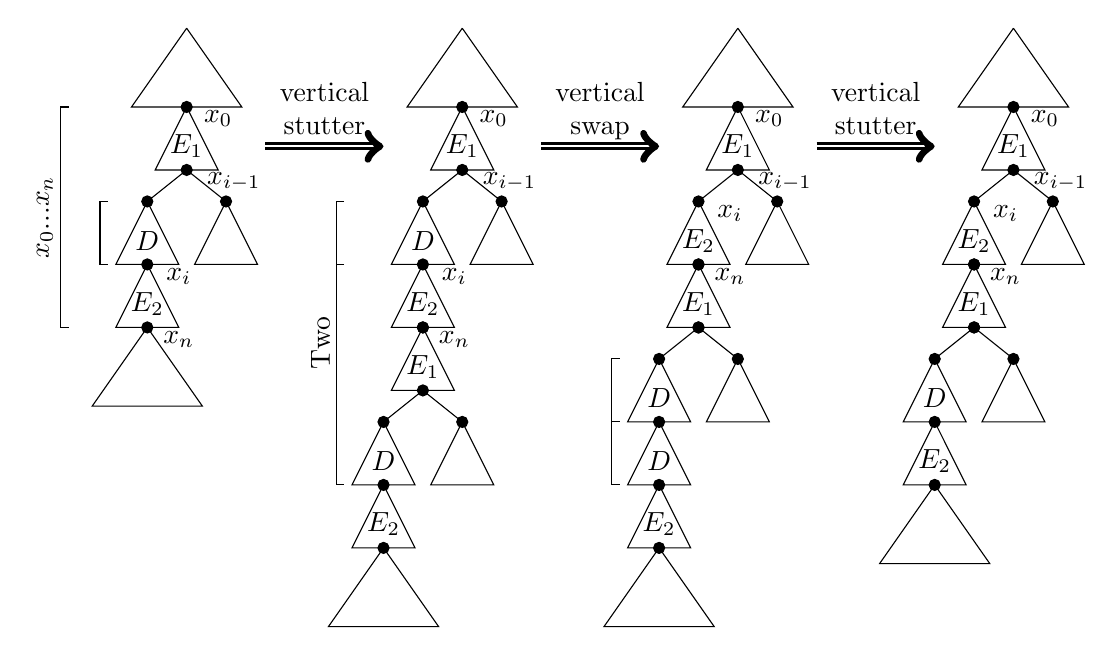
\begin{tikzpicture}




\draw (1.5,9.5) -- (0.8,8.5) -- (2.2,8.5) -- (1.5,9.5);

\draw (1.5,8.5) -- (1.1,7.7) -- (1.9,7.7) -- (1.5,8.5);

\draw (1.0,7.3) -- (1.4,6.5) -- (0.6,6.5) -- (1.0,7.3);
\draw (2.0,7.3) -- (2.4,6.5) -- (1.6,6.5) -- (2.0,7.3);

\draw (1.0,6.5) -- (1.4,5.7) -- (0.6,5.7) -- (1.0,6.5);

\draw (1.0,5.7) -- (1.7,4.7) -- (0.3,4.7) -- (1.0,5.7);

\node[dot] at (1.5,8.5) {};
\node[dot] at (1.5,7.7) {};
\node[dot] at (1.0,7.3) {};
\node[dot] at (2.0,7.3) {};
\node[dot] at (1.0,6.5) {};
\node[dot] at (1.0,5.7) {};

\draw (1.5,7.7) -- (1.0,7.3);
\draw (1.5,7.7) -- (2.0,7.3);


\node[bag] at (1.9,8.35) {$x_{0}$};
\node[bag] at (2.1,7.55) {$x_{i-1}$};

\node[bag] at (1.4,6.35) {$x_{i}$};
\node[bag] at (1.4,5.55) {$x_{n}$};


\node[bag] at (1.0,6.8) {$D$};
\node[bag] at (1.5,8.0) {$E_{1}$};
\node[bag] at (1.0,6.0) {$E_{2}$};


\draw (0.5,7.3) -- (0.4,7.3) -- (0.4,6.5) -- (0.5,6.5);

\draw (0.0,8.5) -- (-0.1,8.5) -- (-0.1,5.7) -- (0.0,5.7);

\node[rotate=90] at (0.2,6.9) {\kloop};


\node[rotate=90] at (-0.3,7.1) {\kloop $x_{0}...x_{n}$};



\draw[double,->,very thick] (2.5,8.0) to node[bag,sloped,above] {\begin{tabular}{c}vertical\\stutter\end{tabular}} (4.0,8.0);





\begin{scope}[xshift=3.5cm]
\draw (1.5,9.5) -- (0.8,8.5) -- (2.2,8.5) -- (1.5,9.5);

\draw (1.5,8.5) -- (1.1,7.7) -- (1.9,7.7) -- (1.5,8.5);

\draw (1.0,7.3) -- (1.4,6.5) -- (0.6,6.5) -- (1.0,7.3);
\draw (2.0,7.3) -- (2.4,6.5) -- (1.6,6.5) -- (2.0,7.3);

\draw (1.0,6.5) -- (1.4,5.7) -- (0.6,5.7) -- (1.0,6.5);

\node[dot] at (1.5,8.5) {};
\node[dot] at (1.5,7.7) {};
\node[dot] at (1.0,7.3) {};
\node[dot] at (2.0,7.3) {};
\node[dot] at (1.0,6.5) {};
\node[dot] at (1.0,5.7) {};

\draw (1.5,7.7) -- (1.0,7.3);
\draw (1.5,7.7) -- (2.0,7.3);


\node[bag] at (1.9,8.35) {$x_{0}$};
\node[bag] at (2.1,7.55) {$x_{i-1}$};

\node[bag] at (1.4,6.35) {$x_{i}$};
\node[bag] at (1.4,5.55) {$x_{n}$};


\node[bag] at (1.0,6.8) {$D$};
\node[bag] at (1.5,8.0) {$E_{1}$};
\node[bag] at (1.0,6.0) {$E_{2}$};


\begin{scope}[xshift=-0.5cm,yshift=-2.8cm]


\draw (1.5,8.5) -- (1.1,7.7) -- (1.9,7.7) -- (1.5,8.5);

\draw (1.0,7.3) -- (1.4,6.5) -- (0.6,6.5) -- (1.0,7.3);
\draw (2.0,7.3) -- (2.4,6.5) -- (1.6,6.5) -- (2.0,7.3);

\draw (1.0,6.5) -- (1.4,5.7) -- (0.6,5.7) -- (1.0,6.5);

\draw (1.0,5.7) -- (1.7,4.7) -- (0.3,4.7) -- (1.0,5.7);

\node[dot] at (1.5,8.5) {};
\node[dot] at (1.5,7.7) {};
\node[dot] at (1.0,7.3) {};
\node[dot] at (2.0,7.3) {};
\node[dot] at (1.0,6.5) {};
\node[dot] at (1.0,5.7) {};

\draw (1.5,7.7) -- (1.0,7.3);
\draw (1.5,7.7) -- (2.0,7.3);





\node[bag] at (1.0,6.8) {$D$};
\node[bag] at (1.5,8.0) {$E_{1}$};
\node[bag] at (1.0,6.0) {$E_{2}$};



\end{scope}
\draw (0.0,7.3) -- (-0.1,7.3) -- (-0.1,3.7) -- (0.0,3.7);
\draw (0.0,6.5) -- (-0.1,6.5);

\node[rotate=90] at (-0.3,5.5) {Two \kloops};


\draw[double,->,very thick] (2.5,8.0) to node[bag,sloped,above] {\begin{tabular}{c}vertical\\swap\end{tabular}} (4.0,8.0);

\end{scope}













\begin{scope}[xshift=7.0cm]
\draw (1.5,9.5) -- (0.8,8.5) -- (2.2,8.5) -- (1.5,9.5);

\draw (1.5,8.5) -- (1.1,7.7) -- (1.9,7.7) -- (1.5,8.5);

\draw (1.0,7.3) -- (1.4,6.5) -- (0.6,6.5) -- (1.0,7.3);
\draw (2.0,7.3) -- (2.4,6.5) -- (1.6,6.5) -- (2.0,7.3);



\node[dot] at (1.5,8.5) {};
\node[dot] at (1.5,7.7) {};
\node[dot] at (1.0,7.3) {};
\node[dot] at (2.0,7.3) {};
\node[dot] at (1.0,6.5) {};
\node[dot] at (1.0,5.7) {};

\draw (1.5,7.7) -- (1.0,7.3);
\draw (1.5,7.7) -- (2.0,7.3);


\node[bag] at (1.9,8.35) {$x_{0}$};
\node[bag] at (2.1,7.55) {$x_{i-1}$};

\node[bag] at (1.4,7.15) {$x_{i}$};
\node[bag] at (1.4,6.35) {$x_{n}$};

\node[bag] at (1.5,8.0) {$E_{1}$};
\node[bag] at (1.0,6.8) {$E_{2}$};


\begin{scope}[xshift=-0.5cm,yshift=-2.0cm]


\draw (1.5,8.5) -- (1.1,7.7) -- (1.9,7.7) -- (1.5,8.5);

\draw (1.0,7.3) -- (1.4,6.5) -- (0.6,6.5) -- (1.0,7.3);
\draw (2.0,7.3) -- (2.4,6.5) -- (1.6,6.5) -- (2.0,7.3);

\draw (1.0,6.5) -- (1.4,5.7) -- (0.6,5.7) -- (1.0,6.5);
\draw (1.0,5.7) -- (1.4,4.9) -- (0.6,4.9) -- (1.0,5.7);


\draw (1.0,4.9) -- (1.7,3.9) -- (0.3,3.9) -- (1.0,4.9);

\node[dot] at (1.5,8.5) {};
\node[dot] at (1.5,7.7) {};
\node[dot] at (1.0,7.3) {};
\node[dot] at (2.0,7.3) {};
\node[dot] at (1.0,6.5) {};
\node[dot] at (1.0,5.7) {};
\node[dot] at (1.0,4.9) {};

\draw (1.5,7.7) -- (1.0,7.3);
\draw (1.5,7.7) -- (2.0,7.3);


\draw (0.5,7.3) -- (0.4,7.3) -- (0.4,5.7) -- (0.5,5.7);
\draw (0.5,6.5) -- (0.4,6.5);


\node[bag] at (1.0,6.8) {$D$};
\node[bag] at (1.5,8.0) {$E_{1}$};
\node[bag] at (1.0,6.0) {$D$};
\node[bag] at (1.0,5.2) {$E_{2}$};



\end{scope}

\draw[double,->,very thick] (2.5,8.0) to node[bag,sloped,above] {\begin{tabular}{c}vertical\\stutter\end{tabular}} (4.0,8.0);
\end{scope}



















\begin{scope}[xshift=10.5cm]
\draw (1.5,9.5) -- (0.8,8.5) -- (2.2,8.5) -- (1.5,9.5);

\draw (1.5,8.5) -- (1.1,7.7) -- (1.9,7.7) -- (1.5,8.5);

\draw (1.0,7.3) -- (1.4,6.5) -- (0.6,6.5) -- (1.0,7.3);
\draw (2.0,7.3) -- (2.4,6.5) -- (1.6,6.5) -- (2.0,7.3);



\node[dot] at (1.5,8.5) {};
\node[dot] at (1.5,7.7) {};
\node[dot] at (1.0,7.3) {};
\node[dot] at (2.0,7.3) {};
\node[dot] at (1.0,6.5) {};
\node[dot] at (1.0,5.7) {};

\draw (1.5,7.7) -- (1.0,7.3);
\draw (1.5,7.7) -- (2.0,7.3);


\node[bag] at (1.9,8.35) {$x_{0}$};
\node[bag] at (2.1,7.55) {$x_{i-1}$};

\node[bag] at (1.4,7.15) {$x_{i}$};
\node[bag] at (1.4,6.35) {$x_{n}$};

\node[bag] at (1.5,8.0) {$E_{1}$};
\node[bag] at (1.0,6.8) {$E_{2}$};


\begin{scope}[xshift=-0.5cm,yshift=-2.0cm]


\draw (1.5,8.5) -- (1.1,7.7) -- (1.9,7.7) -- (1.5,8.5);

\draw (1.0,7.3) -- (1.4,6.5) -- (0.6,6.5) -- (1.0,7.3);
\draw (2.0,7.3) -- (2.4,6.5) -- (1.6,6.5) -- (2.0,7.3);

\draw (1.0,6.5) -- (1.4,5.7) -- (0.6,5.7) -- (1.0,6.5);


\draw (1.0,5.7) -- (1.7,4.7) -- (0.3,4.7) -- (1.0,5.7);

\node[dot] at (1.5,8.5) {};
\node[dot] at (1.5,7.7) {};
\node[dot] at (1.0,7.3) {};
\node[dot] at (2.0,7.3) {};
\node[dot] at (1.0,6.5) {};
\node[dot] at (1.0,5.7) {};

\draw (1.5,7.7) -- (1.0,7.3);
\draw (1.5,7.7) -- (2.0,7.3);





\node[bag] at (1.0,6.8) {$D$};
\node[bag] at (1.5,8.0) {$E_{1}$};
\node[bag] at (1.0,6.0) {$E_2$};



\end{scope}


\end{scope}















\end{tikzpicture}
\end{center}
\caption{The construction of $t_2$, eliminating the context $D$ between
  $x_{i-1}$ and $x_i$}\label{figure-construct-t2}
\end{figure}

 Repeating this argument yields the desired
  tree $t_2$.
 
Consider now the context $C'=t_2[x_0,x_n]$. It is a loop of \ktype $\tau$. Let
$T'$ be the tree constructed from $t$ by inserting $C'$ at $x$. 

\begin{claim} \label{claim-reverse-swaps}
$T' \in L$ iff $t\in L$.
\end{claim}

\begin{proof}
  Consider the sequence of $k$-guarded swaps and $k$-guarded vertical stutter
  that was used in order to obtain $t_2$ from $t$. Because $L$ is \ktame, $t
  \in L$ iff $t_2 \in L$.

  We can easily identify the nodes of $t$ with the nodes of $T'$ outside of
  $C'$. Consider the same sequence of $k$-guarded operations applied to $T'$.
  Observe that this yields a tree $T_2$ corresponding to $t_2$ with possibly several
  extra copies of $C'$. As $C'$ is a \kloop, each of the roots and the ports of these
  extra copies have the same \ktype. Hence, using appropriate vertical $k$-swaps or
  appropriate horizontal $k$-swaps, depending on whether two copies are related or
  not by the descendant relation, they can be brought together. Two examples of
  such operation is given in Figure~\ref{figure-elim-loops}.





\begin{figure}
\begin{center}
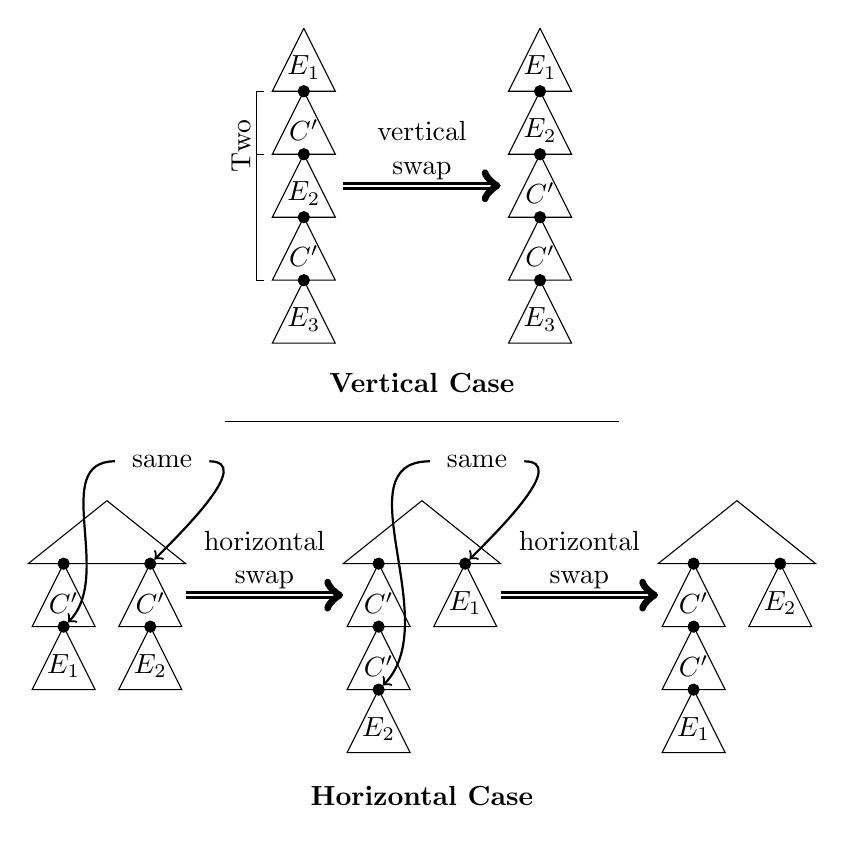
\begin{tikzpicture}




\draw (1.5,8.5) -- (1.1,7.7) -- (1.9,7.7) -- (1.5,8.5);
\draw (1.5,7.7) -- (1.1,6.9) -- (1.9,6.9) -- (1.5,7.7);
\draw (1.5,6.9) -- (1.1,6.1) -- (1.9,6.1) -- (1.5,6.9);
\draw (1.5,6.1) -- (1.1,5.3) -- (1.9,5.3) -- (1.5,6.1);
\draw (1.5,5.3) -- (1.1,4.5) -- (1.9,4.5) -- (1.5,5.3);


\node[dot] at (1.5,7.7) {};
\node[dot] at (1.5,6.9) {};
\node[dot] at (1.5,6.1) {};
\node[dot] at (1.5,5.3) {};

\node[bag] at (1.5,8.0) {$E_1$};
\node[bag] at (1.5,7.2) {$C'$};
\node[bag] at (1.5,6.4) {$E_{2}$};
\node[bag] at (1.5,5.6) {$C'$};
\node[bag] at (1.5,4.8) {$E_{3}$};


\draw (1.0,7.7) -- (0.9,7.7) -- (0.9,5.3) -- (1.0,5.3);
\draw (1.0,6.9) -- (0.9,6.9);

\node[rotate=90] at (0.7,7.0) {Two \kloops};






\draw[double,->,very thick] (2.0,6.5) to node[bag,sloped,above] {\begin{tabular}{c}vertical\\swap\end{tabular}} (4.0,6.5);







\begin{scope}[xshift=3cm]
\draw (1.5,8.5) -- (1.1,7.7) -- (1.9,7.7) -- (1.5,8.5);
\draw (1.5,7.7) -- (1.1,6.9) -- (1.9,6.9) -- (1.5,7.7);
\draw (1.5,6.9) -- (1.1,6.1) -- (1.9,6.1) -- (1.5,6.9);
\draw (1.5,6.1) -- (1.1,5.3) -- (1.9,5.3) -- (1.5,6.1);
\draw (1.5,5.3) -- (1.1,4.5) -- (1.9,4.5) -- (1.5,5.3);


\node[dot] at (1.5,7.7) {};
\node[dot] at (1.5,6.9) {};
\node[dot] at (1.5,6.1) {};
\node[dot] at (1.5,5.3) {};

\node[bag] at (1.5,8.0) {$E_1$};
\node[bag] at (1.5,7.2) {$E_2$};
\node[bag] at (1.5,6.4) {$C'$};
\node[bag] at (1.5,5.6) {$C'$};
\node[bag] at (1.5,4.8) {$E_{3}$};

\end{scope}

\node[bag] at (3.0,4.0) {\bf Vertical Case};

\draw (0.5,3.5) -- (5.5,3.5);


\begin{scope}[xshift=-2.5cm,yshift=-1cm]

\draw (1.5,3.5) -- (0.5,2.7) -- (2.5,2.7) -- (1.5,3.5);

\draw (0.95,2.7) -- (0.55,1.9) -- (1.35,1.9) -- (0.95,2.7);
\draw (0.95,1.9) -- (0.55,1.1) -- (1.35,1.1) -- (0.95,1.9);

\draw (2.05,2.7) -- (1.65,1.9) -- (2.45,1.9) -- (2.05,2.7);
\draw (2.05,1.9) -- (1.65,1.1) -- (2.45,1.1) -- (2.05,1.9);


\node[dot] at (0.95,2.7) {};
\node[dot] (s1) at (0.95,1.9) {};
\node[dot] (s2) at (2.05,2.7) {};
\node[dot] at (2.05,1.9) {};

\node[bag] at (0.95,2.2) {$C'$};
\node[bag] at (0.95,1.4) {$E_1$};
\node[bag] at (2.05,2.2) {$C'$};
\node[bag] at (2.05,1.4) {$E_2$};

\node[bag] (id) at (2.2,4.0) {\begin{tabular}{c}same\\ \ktype \end{tabular}};

\draw[->,thick] (id) to [out=180,in=45] (s1);
\draw[->,thick] (id) to [out=0,in=45] (s2);

\draw[double,->,very thick] (2.5,2.3) to node[bag,sloped,above] {\begin{tabular}{c}horizontal\\swap\end{tabular}} (4.5,2.3);


\end{scope}

\begin{scope}[xshift=1.5cm,yshift=-1cm]

\draw (1.5,3.5) -- (0.5,2.7) -- (2.5,2.7) -- (1.5,3.5);

\draw (0.95,2.7) -- (0.55,1.9) -- (1.35,1.9) -- (0.95,2.7);
\draw (0.95,1.9) -- (0.55,1.1) -- (1.35,1.1) -- (0.95,1.9);
\draw (0.95,1.1) -- (0.55,0.3) -- (1.35,0.3) -- (0.95,1.1);

\draw (2.05,2.7) -- (1.65,1.9) -- (2.45,1.9) -- (2.05,2.7);



\node[dot] at (0.95,2.7) {};
\node[dot] at (0.95,1.9) {};
\node[dot] (s2) at (2.05,2.7) {};
\node[dot] (s1) at (0.95,1.1) {};

\node[bag] at (0.95,2.2) {$C'$};
\node[bag] at (0.95,1.4) {$C'$};
\node[bag] at (2.05,2.2) {$E_1$};
\node[bag] at (0.95,0.6) {$E_2$};

\node[bag] (id) at (2.2,4.0) {\begin{tabular}{c}same\\ \ktype \end{tabular}};

\draw[->,thick] (id) to [out=180,in=45] (s1);
\draw[->,thick] (id) to [out=0,in=45] (s2);


\draw[double,->,very thick] (2.5,2.3) to node[bag,sloped,above] {\begin{tabular}{c}horizontal\\swap\end{tabular}} (4.5,2.3);


\end{scope}

\begin{scope}[xshift=5.5cm,yshift=-1cm]

\draw (1.5,3.5) -- (0.5,2.7) -- (2.5,2.7) -- (1.5,3.5);

\draw (0.95,2.7) -- (0.55,1.9) -- (1.35,1.9) -- (0.95,2.7);
\draw (0.95,1.9) -- (0.55,1.1) -- (1.35,1.1) -- (0.95,1.9);
\draw (0.95,1.1) -- (0.55,0.3) -- (1.35,0.3) -- (0.95,1.1);

\draw (2.05,2.7) -- (1.65,1.9) -- (2.45,1.9) -- (2.05,2.7);



\node[dot] at (0.95,2.7) {};
\node[dot] at (0.95,1.9) {};
\node[dot] at (2.05,2.7) {};
\node[dot] at (0.95,1.1) {};

\node[bag] at (0.95,2.2) {$C'$};
\node[bag] at (0.95,1.4) {$C'$};
\node[bag] at (2.05,2.2) {$E_2$};
\node[bag] at (0.95,0.6) {$E_1$};



\end{scope}

\node[bag] at (3.0,-1.25) {\bf Horizontal Case};

\end{tikzpicture}
\end{center}
\caption{Bringing copies of the \kloop $C'$ together in
Claim~\ref{claim-reverse-swaps}}\label{figure-elim-loops}
\end{figure}






Then, using $k$-guarded vertical stutter all but one copy can be eliminated
resulting in $t_2$. Hence $T' \in L$ iff $t_2\in L$ and the claim is
proved. See figure \ref{figure-relat-t2}.
\end{proof}

\begin{figure}
\begin{center}
\psset{unit=.8cm}
\begin{pspicture}(8,6.6)

\rput(0.0,1.0){
\pspolygon(1.5,5.6)(0.2,3.3)(2.8,3.3)
\rput(1.5,4.3){$t$}
}
\pspolygon(1.5,2.3)(0.2,0)(2.8,0)
\rput(1.5,1.0){$T'$}


\rput(0.0,1.0){
\rput(4.0,4.4){$\Longrightarrow$}
\rput(4.0,5.2){$k$- guarded}
\rput(4.0,4.8){operations}
}

\rput(4.0,1.1){$\Longrightarrow$}
\rput(4.0,1.9){$k$- guarded}
\rput(4.0,1.5){operations}



\rput(1.0,1.0){

\pspolygon(5.5,5.6)(4.2,3.3)(6.8,3.3)
\rput(5.5,4.3){$t_{2}$}

}

\rput(1.0,0.0){
\pspolygon(5.5,2.3)(4.2,0)(6.8,0)
\rput(5.5,1.0){$T_{2}$}

}

\rput(1.0,0.5){

\rput(5.5,2.8){\rotateleft{$\Longrightarrow$}}
\rput(6.8,3.2){deletion}
\rput(6.8,2.8){of extra}
\rput(6.8,2.4){copies of $C'$}

}

\end{pspicture}
\end{center}
\caption{Relation with $t_2$}\label{figure-relat-t2}
\end{figure}


It remains to show that $T' \in L$ iff $T \in L$. By construction of $T'$ we
have \lessblocks{C'}{t}{k+1}. Consider now a node $x_i$ in the principal path
of $C'$. Let $T_i$ be the subtree branching out the principal path of $C$ at
$y_i$ and $T'_i$ be the subtree branching out the principal path of $C'$ at
$x_i$. By construction $x_i$ and $y_i$ are of \type{(k+1)} $\tau_i$. Therefore
the roots of $T_i$ and $T'_i$ have the same \ktype. Because
\lessblocks{C'}{t}{k+1} all the \types{(k+1)} of $T'_i$ already appear in the
part of $T'$ outside of $C'$. By hypothesis we also have \lessblocks{T_i}{t}{k+1}.
Hence we can apply Lemma~\ref{claim-transfer-branch} and replacing $T'_i$
with $T_i$ does not affect membership in $L$. A repeated use of that
lemma eventually shows that $T' \in L$ iff $T \in L$.
\end{proof}

\medskip

We return to the proof of Proposition~\ref{lemma-pumping}. Recall that
we have two trees $t,t'$ such that \sameblocks{t}{t'}{\kappa} for $\kappa=
\beta_k + k + 1$. For $l > \kappa$, we want to construct $T,T'$ such that:
 
\begin{enumerate}[(1)]
\item $t \in L$ iff $T \in L$
\item $t' \in L$ iff $T' \in L$
\item \sameblocks{T}{T'}{l}
\end{enumerate}



Recall that the number of \ktypes is $\beta_k$. Therefore, by choice of $\kappa$, in
every branch of a \type{\kappa} one can find at least one \ktype that is repeated.
This provides many \kloops that can be used using Lemma~\ref{lemma-insert-loop}
for obtaining bigger types.

Take $l > \kappa$, we build $T$ and $T'$ from $t$ and $t'$ by inserting \kloops
in $t$ and $t'$ without affecting their membership in $L$ using
Lemma~\ref{lemma-insert-loop}.

  Let $B = \{\tau_{0},...,\tau_{n}\}$ be the set of \ktypes $\tau$ such that
  there is a loop of \ktype $\tau$ in $t$ or in $t'$. For each $\tau \in B$ we
  fix a context $C_\tau$ as follows. Because $\tau \in B$ there is a context
  $C$ in $t$ or $t'$ that is a loop of \ktype $\tau$. For each $\tau \in B$, we
  fix arbitrarily such a $C$ and set $C_\tau$ as $\underbrace{C \cdot \ldots
    \cdot C}_{l}$, $l$ concatenations of the context $C$. Notice that the path
  from the root of $C_\tau$ to its port is then bigger than $l$.

  We now describe the construction of $T$ from $t$. The construction of $T'$
  from $t'$ is done similarly. The tree $T$ is constructed by simultaneously inserting,
  for all $\tau \in B$, a copy of the context $C_\tau$ at all nodes of $t$ of type $\tau$.

  We now show that $T$ and $T'$ have the desired properties. 
  
  The first and second properties, $t \in L$ iff $T \in L$ and $t' \in L$ iff
  $T' \in L$, essentially follow from Lemma~\ref{lemma-insert-loop}. We only
  show that $t \in L$ iff $T \in L$, the second property is proved
  symmetrically. We view $T$ as if it was constructed from $t$ using a sequence
  of insertions of some context $C_\tau$ for $\tau \in B$. We write
  $s_0,...,s_m$ the sequence of intermediate trees with $s_0=t$ and $s_m=T$. We
  call $C_i$ the context inserted to get $s_{i+1}$ from $s_{i}$.  We show by
  induction on $i$ that (i) \sameblocks{s_i}{t}{k+1} and (ii) $s_i \in L$ iff
  $s_{i+1}\in L$. This will imply $t \in L$ iff $T \in L$ as desired.  (i) is
  clear for $i=0$. We show that for all $i$ (i) implies (ii). Recall that $C_i$
  is the concatenation of $l$ copies of a \kloop present either in $t$ or in
  $t'$.  We suppose without generality that the \kloop is present in $t$.  Let
  $s$ be the tree constructed from $t$ by duplicating the \kloop $l$
  times. Hence $s$ is a tree containing $C_i$ and by construction
  \sameblocks{s}{t}{k+1}. Because \sameblocks{t}{t'}{\kappa} with $\kappa >
  k+1$ and \sameblocks{s_i}{t}{k+1} we have \sameblocks{s}{s_i}{k+1}. By
  Lemma~\ref{lemma-insert-loop} this implies that $s_{i+1} \in L$ iff $s_{i}
  \in L$. By construction we also have \sameblocks{s_{i+1}}{s_i}{k+1} and the
  induction step is proved.


We now show the third property:

  \begin{lem}\label{claim-sameblock}
    \sameblocks{T}{T'}{l}
  \end{lem}

\proof
  We need to show that \lessblocks{T}{T'}{l}, \lessblocks{T'}{T}{l} and that
  the roots of $T$ and $T'$ have the same \type{l}. It will be convenient for
  proving this to view the nodes of $T$ as the union of the nodes of $t$ plus
  some nodes coming from the \kloops that were inserted. To do this more
  formally, if $x$ is a node of $t$ of \ktype not in $B$, then $x$ is
  identified with the corresponding node of $T$. If $x$ is a node of $t$ whose
  \ktype is in $B$ then $x$ is identified in $T$ with the port of the copy of
  $C_\tau$ that was inserted at node $x$.  We start with the following claim.


  \begin{claim} \label{claim-identify-types} Take two nodes $x$ in $t$ and $x'$
    in $t'$, such that $x$ and $x'$ have the same \type{\kappa}. Let $y$ and $y'$ be
    the corresponding nodes in $T$ and $T'$. Then $y$ and $y'$ have the same
    \type{l}.
\end{claim}


\begin{proof}
  Let $\nu$ the \type{\kappa} of $x$ and $x'$.  Consider a branch of $\nu$ of
  length $\kappa$. By the choice of $\kappa$ we know that in this branch one
  can find two nodes $z$ and $z'$ with the same \ktypes $\tau$, with $z$ an
  ancestor of $z'$ and such that the \ktype $\tau$ of $z$ is determined by
  $\nu$ ($z$ is at distance $\geq k$ from the leaves of $\nu$). Hence $\tau$ is
  in $B$.  Note that because the \ktype of $z$ is included in $\nu$, the
  presence of a node of type $\nu$ induces the presence of a node of type
  $\tau$ at the same relative position than $z$. Hence a copy of $C_\tau$ is
  inserted simultaneously at the same position relative to $y$ and $y'$ during the
  construction of $T$ and $T'$.  Because this is true for all branches of $\nu$
  and because all $C_\tau$ have depth at least $l$, then $y$ and $y'$ have the
  same \type{l}.
\end{proof}

From claim~\ref{claim-identify-types} it follows that the roots of $T$ and $T'$
have the same \type{l}. By symmetry we only need to show that
\lessblocks{T}{T'}{l}. Let $y$ be a node of $T$ and $\mu$ be its \type{l}. We
show that there exists $y' \in T'$ with type $\mu$. We consider two cases:

\begin{iteMize}{$\bullet$}
\item $y$ is not a node of a loop inserted during the construction of $T$. Let
  $x$ be the corresponding position in $t$ and let $\nu$ be its \type{\kappa}. Since
  \sameblocks{t}{t'}{\kappa}, there is a node $x'$ of $t'$ of type $\nu$. Let $y'$
  be the node of $T'$ corresponding to $y'$. By
  Claim~\ref{claim-identify-types} $y$ and $y'$ have the same \type{l}.

\item $y$ is a node inside a copy of $C_\tau$ inserted to construct $T$. Let $x$ be the
  node of $t$ where this loop was inserted. Let $\nu$ be the \type{\kappa} of $x$ (the \ktype of
  $x$ is $\tau$).  Since \sameblocks{t}{t'}{\kappa}, there is a node $x'$ of $t'$ of
  type $\nu$. Since $\kappa > k$, $x$ and $x'$ have the same \type{k}, a
  copy of $C_\tau$ was also inserted in $t'$ at position $x'$ during the
  construction of $T'$. From Claim~\ref{claim-identify-types}, $x$ and
  $x'$, when viewed as nodes of $T$ and $T'$ have the same \type{l}.  Let $y'$ be the node of $T'$ in the copy of
  $C_\tau$ inserted at $x'$ that corresponds to the position $y$. Since $y$ and
  $y'$ are ancestors of $x$ and $x'$ that have the same \type{l}, and since the
  context from $y$ to $x$ is the same as the context from $y'$ to $x'$, then $y$ and $y'$ must have the same
  \type{l}.\qed
\end{iteMize}

\noindent This concludes the proof of Proposition~\ref{lemma-pumping}.
\end{proof}


